
\documentclass[ms.tex]{subfiles}
\begin{document}

\section{Galactic Properties}
\label{sec:galprops}

% fig 1
\begin{figure*}
\centering
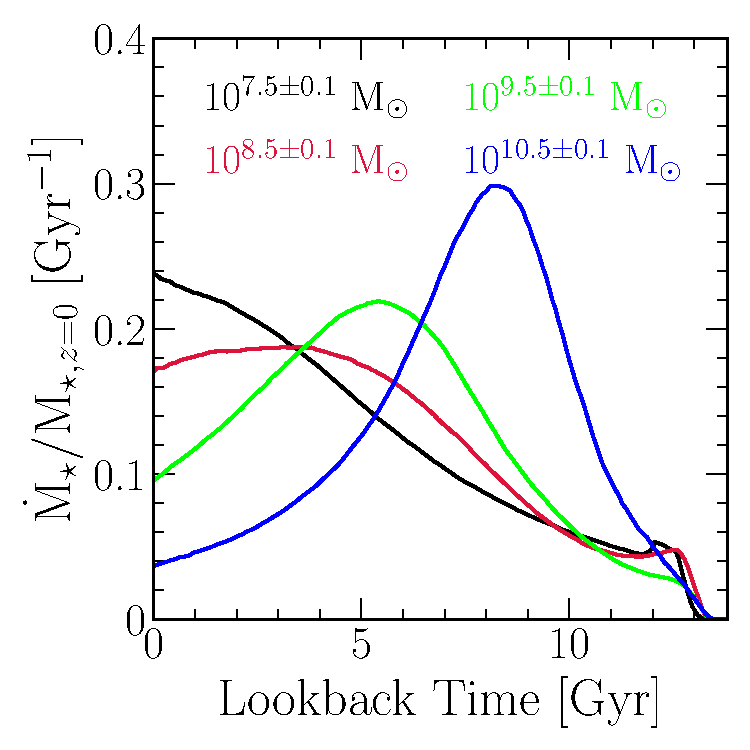
\includegraphics[scale = 0.43]{umachine_sfhs.pdf}
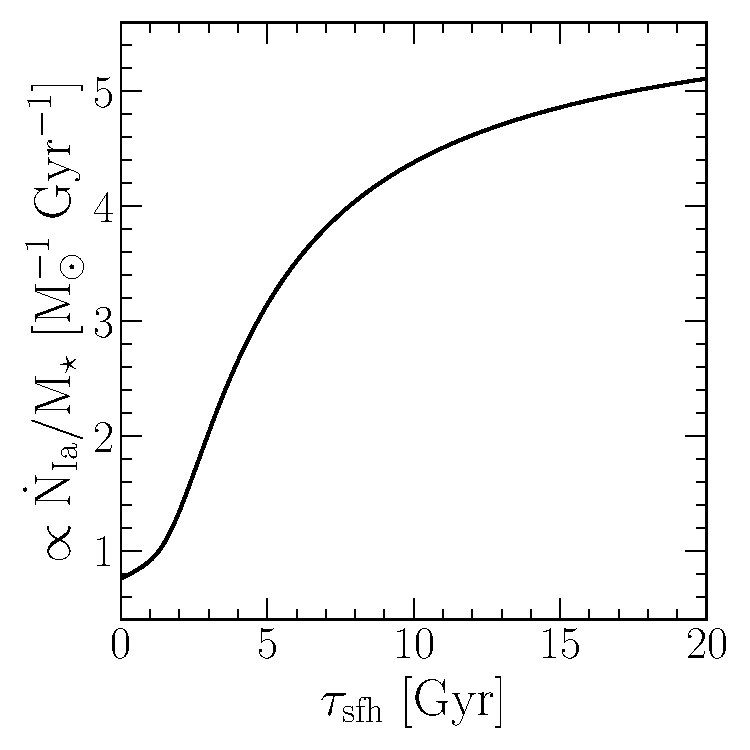
\includegraphics[scale = 0.42]{iarate_vs_tausfh.pdf}
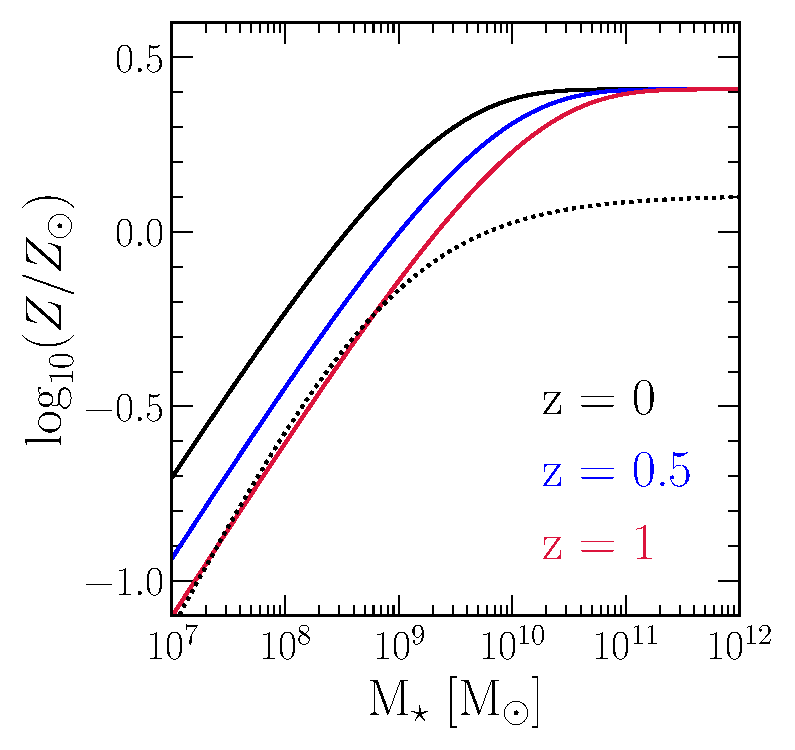
\includegraphics[scale = 0.42]{mzr.pdf}
\caption{
\textbf{Left}: The best-fit mean SFH of galaxies with present-day stellar
masses of $\mstar = 10^{7.5 \pm 0.1}$ (black),~$10^{8.5 \pm 0.1}$ (red),
$10^{9.5 \pm 0.1}$ (green), and $10^{10.5 \pm 0.1} \msun$ (blue) as reported
by~\um~and normalized by the present-day stellar mass itself.
\textbf{Middle}: The specific SN Ia rate as a function of the e-folding
timescale of the SFH~$\tau_\text{sfh}$ assuming a linear-exponential time
dependence and a~$\tau^{-1}$ power-law SN Ia DTD.
\textbf{Right}: The redshift-dependent MZR reported by~\citet{Zahid2014} at
$z = 0$ (black solid),~$z = 0.5$ (blue), and~$z = 1$ (red).
For comparison, we additionally plot the MZR measured by
\citet[][black dotted, appropriate for~$z \approx 0$]{Andrews2013}.
}
\label{fig:sfh_mzr}
\end{figure*}

In this paper, we assume that the strong scaling of the specific SN Ia rate
with stellar mass is due to metallicity effects and conduct simple numerical
calculations to investigate its origin.
We combine the mean star formation histories of galaxies at fixed stellar
mass and the popular~$\tau^{-1}$ SN Ia DTD~\citep[e.g.][]{Maoz2012a}
with the mass-metallicity relation (MZR) for galaxies~\citep{Tremonti2004,
Andrews2013, Zahid2011, Zahid2014}.
With the mean SFH and DTD, we can compute the characteristic SN Ia rate for
galaxies of a given stellar mass, and by assuming that they lie along the
observed MZR, we can simultaneously fold in various scalings with
metallicity~$Z$.
\par
We begin by examining how the mean galactic SFH varies with present-day stellar
mass as predicted by the~\um~semi-analytic model~\citep{Behroozi2019}.
Using dark matter halo properties supplied by the~\textit{Bolshoi-Planck} and
\textit{Multi-Dark Planck 2} dark matter only simulations~\citep{Klypin2016,
RodriguezPuebla2016},~\um~follows a convention semi-analytic model framework
(see, e.g., the review in~\citealt{Somerville2015a}) by parametrizing the SFRs
of galaxies as a function of lookback time, the assembly history of the halo,
and the depth of the halo's potential well.
Like other semi-analytic models that came before it,~\um~successfully
reproduces a broad range of well-constrained observables, including stellar
mass functions, cosmic SFRs, specific SFRs, quenched fractions, UV luminosity
functions, and more.
While some semi-analytic models have used the extended Press-Schechter
formalism~\citep{Press1974, Bond1991} to generate halo merger trees and push
the lower stellar mass limit of their model down to~$\mstar \approx 10^7~\msun$
\citep[e.g.][]{Somerville2015b}, an advantage of~\um~is that the high mass
resolution of~\textit{Bolshoi-Planck} and~\textit{Multi-Dark Planck 2}
allows merger trees down to~$\mstar = 10^{7.2}~\msun$ to be obtained directly
from the simulations.
Dwarf galaxies in this regime are of particular interest to our investigation
because the scaling of the specific SN Ia rate with stellar mass measured by
\citet{Brown2019} extends as low as~$\sim 10^7~\msun$ in their volume-limited
sample and~$\sim 10^6~\msun$ in their full sample.
We therefore examine galaxies from~$\mstar = 10^{7.2} - 10^{12}~\msun$,
spanning the full range of stellar masses for which there are both mean SFHs
available from~\um~and empirical constraints on the SN Ia rate from
ASAS-SN~\citep{Brown2019, Gandhi2022} and DES~\citep{Wiseman2021}.
\par
In the left panel of Fig.~\ref{fig:sfh_mzr}, we plot the best-fit mean SFH as a
function of lookback time in four narrow bins of observed stellar mass taken
from~\um.
In the interest of relating these predictions to data from ASAS-SN
\citep{Shappee2014, Kochanek2017}, an untargeted survey, we take the full
galaxy sample from~\um, including both star forming and quenched galaxies as
well as both centrals and satellites, though centrals are the dominant
population across the full stellar mass range.
In general, low stellar mass galaxies have more extended SFHs than their
higher mass counterparts.
This effect is sufficiently strong such that around~$10^{7.5}~\msun$, typical
SFRs are still increasing at the present day while~$\sim10^{10.5}~\msun$
galaxies experienced their fastest star formation many e-folding timescales ago.
% In principle, this should impact the characteristic SN Ia rate as a function of
% galaxy mass.
\par
Although the details of the SN Ia DTD have been a topic of active inquiry for
some time~\citep[e.g.][]{Greggio2005, Strolger2020, Freundlich2021},
comparisons of the cosmic SFH~\citep[e.g.][]{Hopkins2006, Davies2016, Madau2014,
Madau2017, Driver2018} with the volumetric SN Ia rate as a function of redshift
suggest that the cosmic DTD is broadly consistent with a~$\tau^{-1}$ power-law
(\citealp{Maoz2012a};~\citealp*{Maoz2012b};~\citealp{Graur2013, Graur2014}).
A DTD of approximately this form is also expected under the double-degenerate
scenario given population synthesis models of binary white dwarfs and the loss
of angular momentum due to graviational wave emission (e.g.
\citealp{Mennekens2010};~\citealp*{Maoz2014}).
We therefore adopt this parametrization in this paper, though we have
reconducted our analysis using an exponential DTD with a timescale of
$\tau_\text{Ia} = 1.5$ Gyr and found similar results.
We do not consider metallicity-dependent variations in the shape of the DTD
here, instead focusing on the overall normalization.
\par
In principle, the minimum delay time of the DTD could be as short as~$\sim$40
Myr if WDs are produced by~$\lesssim 8~\msun$ stars~\citep*[e.g.][]{Hurley2000},
and perhaps even shorter at low metallicity if the total metal content of a
star significantly impacts its lifetime as in, e.g.,~\citet{Kodama1997} and
\citet{Vincenzo2016}.
However, if SNe Ia require some additional time following WD formation, the
minimum delay will be longer.
Since we are interested in demonstratin the first-order effects of variations
in SFHs on specific SN Ia rates, we assume a value of~$t_\text{D} = 100$ Myr.
We have also reproduced the results of this paper with both~$t_\text{D} = 40$
Myr and~$t_\text{D} = 150$ Myr and found similar results in both cases.
\par
For an SFH~$\dot{M}_\star$ and DTD~$R_\text{Ia}$ as functions of lookback time
$\tau$, the specific SN Ia rate at some stellar mass~$\mstar$ can be expressed
as
\begin{equation}
\frac{\dot{N}_\text{Ia}(M_\star | \gamma)}{M_\star} = Z(M_\star)^\gamma
\ddfrac{
	\int_0^{T - t_\text{D}}\dot{M}_\star(\tau | M_\star) R_\text{Ia}(\tau) d\tau
}{
	(1 - f_\text{loss})\int_0^T \dot{M}_\star(\tau | M_\star) d\tau
}
\label{eq:specia}
\end{equation}
where~$T$ is the time elapsed between the onset of star formation and the
present day and~$f_\text{loss}$ is a corrective term to account for mass loss
as stellar populations age.
Visual inspection of the left panel of Fig.~\ref{fig:sfh_mzr} indicates that
$T \approx 13.2$ Gyr across this broad range of stellar masses; we therefore
make this assumption throughout this paper.
To investigate scalings with metallicity of various strengths, we artificially
introduce the single-component power-law~$Z^\gamma$ where~$Z$ is given by the
MZR.
While the normalization of the SFH cancels, we omit the normalization of the
DTD from equation~\refp{eq:specia} because we are not interested in the
absolute SN Ia rate in the present paper -- only the relative scaling as a
function of galaxy stellar mass.
In detail,~$f_\text{loss}$ varies with the age of a stellar population.
However, the material that is eventually returned to the ISM is dominated by
high mass stars with short lifetimes, and the loss rate drops rapidly to the
long lifetimes of lower mass stars.
It is therefore accurate to first-order to assume that stellar populations of
all ages have returned~$f_\text{loss} \approx 40\%$ of their initial mass back
to the ISM (appropriate for a~\citealt{Kroupa2001} IMF;
$f_\text{loss} \approx 20\%$ for a~\citealt{Salpeter1955} IMF; see discussion
in~\S\S~2.2 and 3.7 of~\citealt*{Weinberg2017}).
Although the present-day stellar mass~$\mstar$ is known~\textit{a priori} to
equation~\refp{eq:specia}, the stellar masses at intermediate times are
necessary for our investigation of the redshift evolution of the specific SN Ia
rate in~\S~\ref{sec:diagnostics} below.

% fig 2
\begin{figure*}
\centering
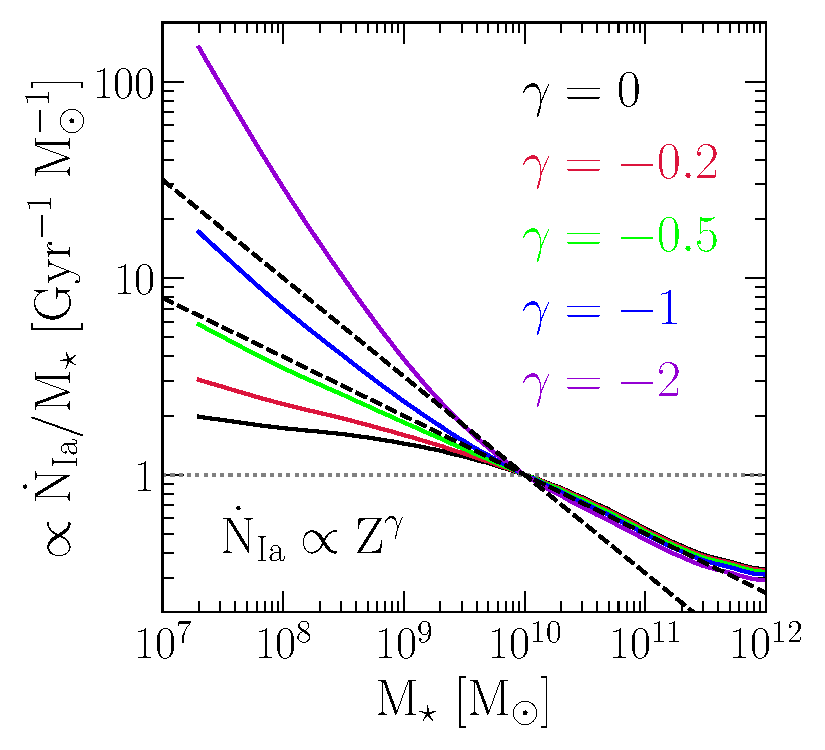
\includegraphics[scale = 0.55]{umachine_iarate_metdep.pdf}
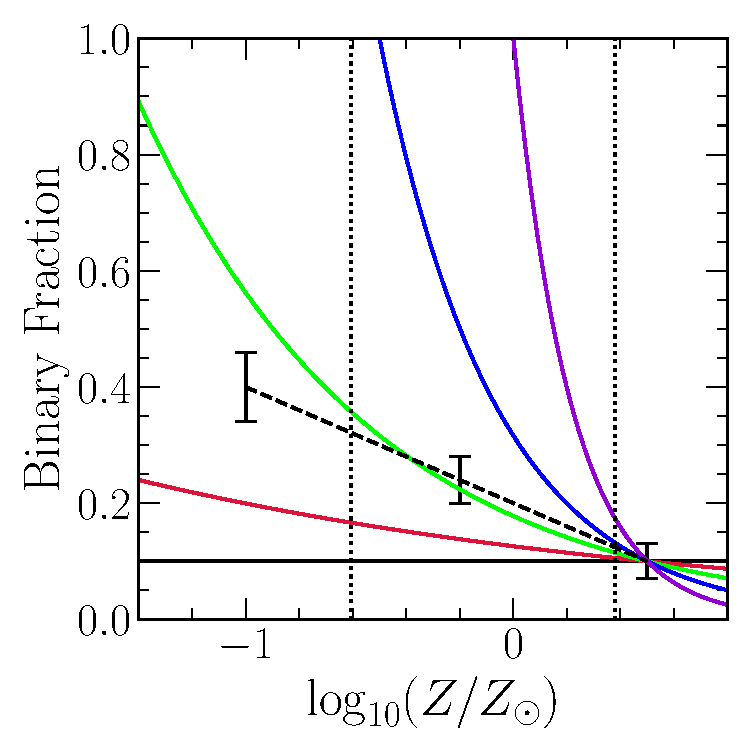
\includegraphics[scale = 0.56]{binaries_zscaling.pdf}
\caption{
\textbf{Left}: Theoretically predicted scalings of the specific SN Ia rate with
galaxy stellar mass (see equation~\ref{eq:specia}) assuming the mean SFHs
reported by~\um~and a single power-law dependence on metallicity~$Z^\gamma$
with~$\gamma = 0$ (i.e. no dependence; black),~$\gamma = -0.2$ (red),
$\gamma = -0.5$ (green),~$\gamma = -1$ (blue), and~$\gamma = -2$ (purple).
Following~\citet{Brown2019} and~\citet{Gandhi2022}, we normalize all rates to
a value of 1 at~$\mstar = 10^{10}~\msun$.
\textbf{Right}: The same metallicity scalings as in the left panel in
comparison to the close binary fractions observed in APOGEE
\citep[][black dashed line with error bars]{Moe2019}.
All metallicity scalings are normalized to the observed binary fraction of 10\%
at~$\log_{10}(Z / Z_\odot) = +0.5$.
We mark the characteristic metallicity of a~$\mstar = 10^{7.2}~\msun$ galaxy
($\log_{10}(Z / Z_\odot) \approx -0.6$) according to the~\citet{Zahid2014} MZR
with a black dotted line.
}
\label{fig:specia_metdep}
\end{figure*}

To qualitatively illustrate how the specific SN Ia rate scales with how prompt
or extended the SFH is, we consider the simple example of a linear-exponential
parametrization~$\dot{M}_\star \propto te^{-t/\tau_\text{sfh}}$ where
$t = T - \tau$.
The middle panel of Fig.~\ref{fig:sfh_mzr} shows equation~\refp{eq:specia} as
a function of the e-folding timescale~$\tau_\text{sfh}$ assuming~$\gamma = 0$.
The specific SN Ia rate is slowest in the limiting case of a single episode of
star formation (i.e.~$\tau_\text{sfh} = 0$) and rises steeply until
$\tau_\text{sfh} \approx 10$ Gyr.
The rate is less sensitive to longer e-folding timescales as the galaxy is
approaching the regime in which its SFH is approximately constant
(i.e.~$\tau_\text{sfh} \gg T$).
Although a~$\tau^{-1}$ DTD is significantly extended (more so than a single
exponential), it is not so extended such that galaxies with sharply declining
SFHs can sustain high SN Ia rates from the earliest epochs of star formation.
A higher specific SN Ia rate as observed in dwarf galaxies is therefore a
natural consequence of their more extended SFHs, though we demonstrate below
that this effect accounts for only a factor of~$\sim$2 between~$10^{7.2}$ and
$10^{10} \msun$.
\par
Not only do dwarf galaxies have more extended SFHs, but the empirical MZR
indicates that they also have a lower metal content~\citep{Tremonti2004,
Gallazzi2005, Zahid2011, Kirby2013}.
At low metallicities, there are multiple effects which could increase the SN Ia
rate.
At fixed initial mass, low metallicity stars leave behind more massive WDs due
to weaker winds and consequently enhanced core growth during the AGB phase
\citep{Umeda1999, Willson2000, Marigo2007, Meng2008, Zhao2012, Kalirai2014}.
This effect could make it easier for a WD to reach the Chandrasekhar mass and
explode (see discussion in~\citealt{Kistler2013}).
Additionally, the stellar close binary fraction is known to increase from
$\sim$10\% at~$\sim$3 times the metallicity of the sun~$Z_\odot$ to~$\sim$40\%
at~$\sim0.1 Z_\odot$~\citep{Moe2019}.
Consequently, dwarf galaxies should have more potential SN Ia progenitors per
unit mass of star formation due to more massive WDs and a higher close binary
fraction.
\par
In the right panel of Fig.~\ref{fig:sfh_mzr} we plot the MZR at a selection of
redshifts as parametrized by
\citet[][see their equation 5]{Zahid2014}.\footnote{
	We have transformed from their~$\log_{10}\text{(O/H)}$ measurements to the
	logarithmic abundance relative to the sun~$\log_{10}(Z / Z_\odot)$ assuming
	the solar oxygen abundance derived by~\citet{Asplund2009}.
}
Although~\um~allows us to investigate these effects at stellar masses as low as
$10^{7.2}~\msun$,~\citet{Zahid2014} present measurements only for the
$\mstar \approx 10^9 - 10^{11}~\msun$ range.
We have therefore reconducted our analysis at~$z = 0$ using the parametric form
of~\citet{Andrews2013}.
They use stacked spectra from the seventh data release of the Sloan Digital
Sky Survey~\citep[SDSS;][]{York2000, Abazajian2009, Abdorrouf2022} to increase
the signal-to-noise of the weak [OII] and [OIII] auroral lines at 7320, 7330
and 4363~\AA~to obtain direct measurements of the electron temperatures and
abundances in bins of stellar mass extended as low as~$\sim 10^{7.4}~\msun$.
We show the~\citet{Andrews2013} MZR in comparison to the~\citet{Zahid2014} form
in the right panel of Fig.~\ref{fig:sfh_mzr}.
The~\citet{Andrews2013} parametrization has a lower plateau but otherwise a
similar slope and turnover mass.
Although neither~\citet{Andrews2013} nor~\citet{Zahid2014} measure the MZR
above~$10^{11}~\msun$, both suggest that these galaxies should be on the
plateau anyway.
We find similar results in~\S~\ref{sec:predictions} below using both
parametrizations because, following~\citet{Brown2019} and~\citet{Gandhi2022},
we quantify the specific SN Ia rate as a function of stellar mass normalized to
1 at~$10^{10}~\msun$.
Therefore, the normalization of the MZR is irrelevant and what determines the
mass dependence in our calculations is the metallicity relative to that of
a~$10^{10}~\msun$ galaxy.
In the interest of exploring SN Ia rates at redshifts of~$z = 0.5$ and~$z = 1$,
we retain the~\citet{Zahid2014} formalism in~\S\S~\ref{sec:predictions}
and~\ref{sec:diagnostics} below.

\end{document}
